%++++++++++++++++++++++++++++++++++++++++
% Don't modify this section unless you know what you're doing!
\documentclass[letterpaper,11pt,ngerman]{article}
%++++
%+++
\usepackage{fontspec}
\usepackage{polyglossia}
\setmainlanguage[babelshorthands=true]{german}
\usepackage{siunitx}
\usepackage{longtable,booktabs}
\usepackage{varwidth}
\usepackage{avant} % Use the Avantgarde font for headings
%\usepackage{times} % Use the Times font for headings
\usepackage{mathptmx} % Use the Adobe Times Roman as the default text font together with math symbols from the Sym­bol, Chancery and Com­puter Modern fonts
\usepackage{xcolor}
\usepackage{microtype} % Slightly tweak font spacing for aesthetics
\usepackage[utf8]{inputenc} % Required for including letters with accents
\usepackage{amssymb}
\usepackage{tabularx} % extra features for tabular environment
\usepackage{amsmath}  % improve math presentation
\usepackage{graphicx} % takes care of graphic including machinery
\usepackage[margin=1in,letterpaper]{geometry} % decreases margins
\usepackage{float}
\usepackage[nohyperlinks, printonlyused, withpage, smaller]{acronym}
% \usepackage{bibgerm} % Literatur in Deutscher DIN
\usepackage[
backend=biber,
style=numeric,
sorting=ynt
]{biblatex}
\addbibresource{bibliography.bib}
\usepackage{subfigure}
\usepackage[final]{hyperref} % adds hyper links inside the generated pdf file
\usepackage{titlesec}
\usepackage{wrapfig,lipsum,booktabs}
\usepackage{setspace}
\usepackage{url}
\hypersetup{
	colorlinks=true,       % false: boxed links; true: colored links
	linkcolor=black,        % color of internal links
	citecolor=black,        % color of links to bibliography
	filecolor=magenta,     % color of file links
	urlcolor=blue
}

\usepackage{blindtext}
\usepackage{cleveref}

\setlength{\parindent}{0pt} % disable paragraph indent

%++++++++++++++++++++++++++++++++++++++++
\let\subsectionautorefname\sectionautorefname
\let\subsubsectionautorefname\sectionautorefname

\titleformat*{\section}{\LARGE\bfseries}
\titleformat*{\subsection}{\Large\bfseries}
\titleformat*{\subsubsection}{\large\bfseries}

\begin{document}
\title{Handout}

\begin{center}
\huge
  	Technische Hochschule Ingolstadt \\
  	\vspace{5mm}
 	
\includegraphics[height=3cm]{TH-Ingolstadt.png}\\
  	\vspace{20mm}
  	Dokumentation zum Projekt\\
  	\vspace{30mm}
  	Thema:\\
  	Implementierung des 802.11p-Standards auf einer Wireless Open-Access Research Platform\\

  	\vspace{70mm}
  	\large
  \begin{tabular}{rcl}
         $$Authoren $$ &:& $$Dominik Bayerl und Philipp Sebastian Schmieder$$ \\
         $$Studiengang$$ &:& $$Master Informatik$$\\
         $$Betreuende Professoren:$$ &:& $$Prof. Dr.-Ing. Ernst-Heinrich Göldner und Prof. Dr. Stefan Hahndel$$ \\
         $$Im Fach$$ &:& $$IM\_Projekt$$\\
         $$Semester$$ &:& $$Wintersemester 2017/2018$$\\
      \end{tabular}
   \end{center}
  \normalsize
  \thispagestyle{empty}
\newpage
\Large

\begin{figure}[H]
%\includegraphics[height=1.8cm,width=8cm]{Unterschrift.jpg}
\end{figure}

\thispagestyle{empty}
\newpage
\tableofcontents
\thispagestyle{empty}
\newpage

\section*{Abkürzungsverzeichnis}
\begin{acronym}[IP-Core]
% Chapter 2
\acro{ofdm}[OFDM]{Orthogonal Frequency-Division Multiplexing}
\acro{fpga}[FPGA]{Field Programmable Gate Array}
\acro{spi}[SPI]{Serial Peripheral Interface}
\acro{rf}[RF]{Radio Frequency}
\acro{adc}[ADC]{Analog Digital Converter}
\acro{dac}[DAC]{Digital Analog Converter}
\acro{dlt}[DLT]{Data Link Type}

% Chapter 3
\acro{cfo}[CFO]{Center Frequency Offset}
\acro{dma}[DMA]{Direct Memory Access}
\acro{fpga}[FPGA]{Field Programmable Gate Array}
\acro{fifo}[FIFO]{First in First out}
\acro{ip-core}[IP-Core]{Intellectual Property Core}
\acro{lts}[LTS]{Long training sequence}
\acro{pll}[PLL]{Phase-locked Loop}
\acro{rf}[RF]{Radio Frequency}
\end{acronym}
\newpage

\setcounter{page}{1}
\begin{onehalfspace}
\section{Projektbeschreibung und Anmerkungen}
\small Author: Philipp Sebastian Schmieder\\
\Large
In diesem Projekt soll der IEEE 802.11p-Standard auf einer Wireless Open-Access Research Platform implementiert werden. 802.11p ist der festgelegte Wireless Kommunikationsstandard für die Car2x Kommunikation. Zum Ende des Projekts soll es möglich sein die Plattform mit kommerziellen 802.11p Geräten kommunizieren zu lassen. Die folgenden Kapitel beschreiben die Grundlagen die zur Umsetzung einer Wireless Kommunikation auf der Wireless Open-Access Research Platform wichtig sind, dabei wird ein Überblick über die Hardware und über die vorhandene Software gegeben. Um dem Leser später den 802.11p-Standard näher zu bringen, wird der als Software für die Plattform bereits umgesetzte 802.11a-Standard mit dem 802.11p-Standard verglichen und die Unterschiede in der physikalischen Schicht verdeutlicht. Die weiteren Kapitel befassen sich mit der Umsetzung des Standards auf der Plattform und der Validierung der Ergebnisse. Als letztes wird ein Ausblick gegeben welche Optimierungsmöglichkeiten in Zukunft noch vorgenommen werden können und wie die Plattform noch erweitert werden könnte.
\section{Die Wireless Open-Access Research Platform}
\small Author: Philipp Sebastian Schmieder\\
\Large
Die Wireless Open-Access Research Platform, kurz WARP, ist eine ständig weiterentwickelte frei verfügbare Plattform zur Entwicklung von Wireless Applikationen und Netzwerken.
Die Plattform kombiniert eine hochperformante Hardware mit diversen Referenz Software Designs die für eigene Anwendungen angepasst oder weiterentwickelt werden können.
\subsection{Das WARP v3 Kit}
\label{sec:hardware}
\begin{figure}[H]
\begin{center}
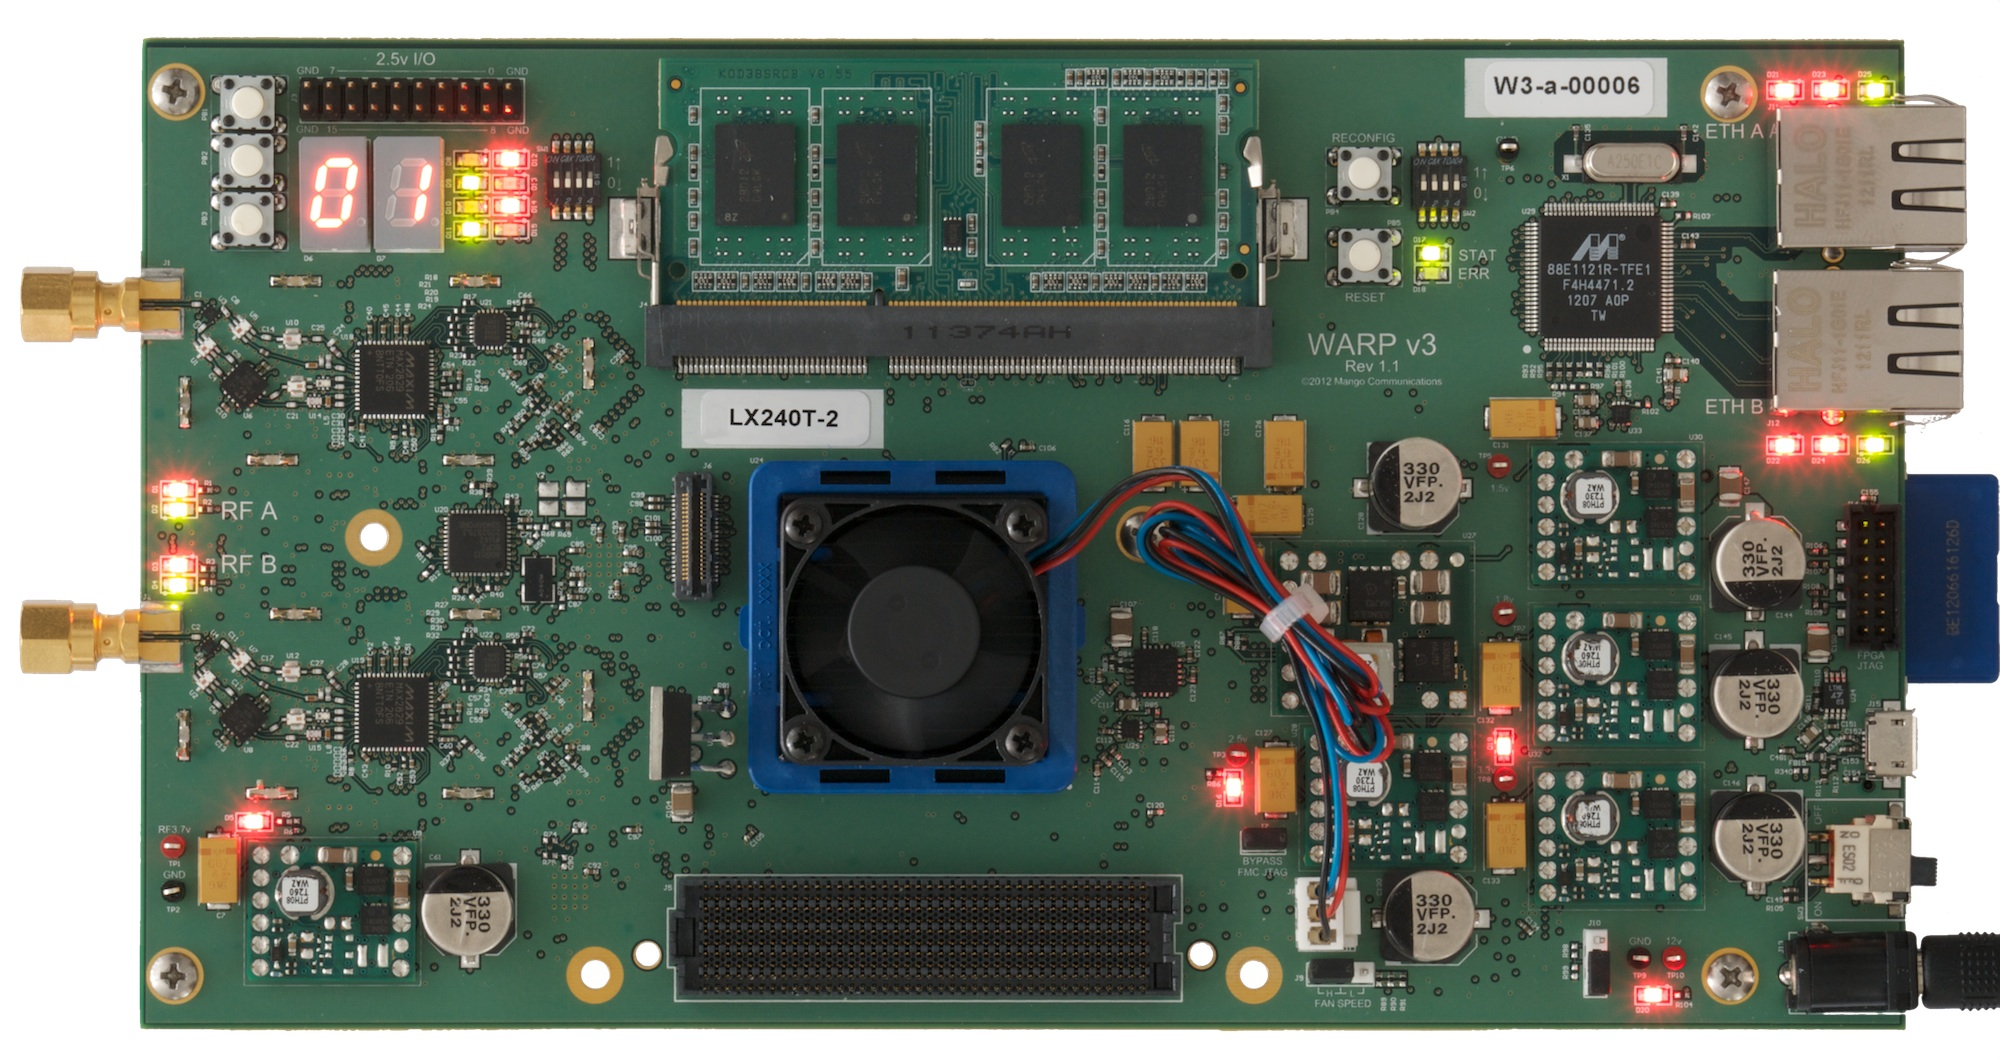
\includegraphics[width = 16cm,height=8cm]{w3_kit_med.jpg}
\caption{Die Warp Hardware von Mango Communications \cite{[2]}}
\label{fig11}
\end{center}
\end{figure}
\noindent Das Mango v3 Kit ist die bisher neueste Hardware Version für die Plattform (Stand: Dezember 2017), das Kit verfügt über einen hochperformanten Virtex-6 FPGA von Xilinx. Zur Konfiguration des FPGA verfügt das Kit über diverse Schnittstellen wie JTAG und einen SD-Karten Stecker. Das FPGA ist volatile, das heißt es muss nach jedem Ausschalten beim Neustart neu konfiguriert werden. Des weiteren verfügt das v3 Kit noch über 2 Gigabit Ethernet Schnittstellen, eine U-Art Schnittstelle,diverse Speicher und Spannungsbauteile, zwei Oszillatoren und 2 baugleiche Radio Frequency (RF) Interfaces.
\subsection{Konfiguration des RF Interfaces}
\label{ssc:RF}
\begin{figure}[H]
\begin{center}
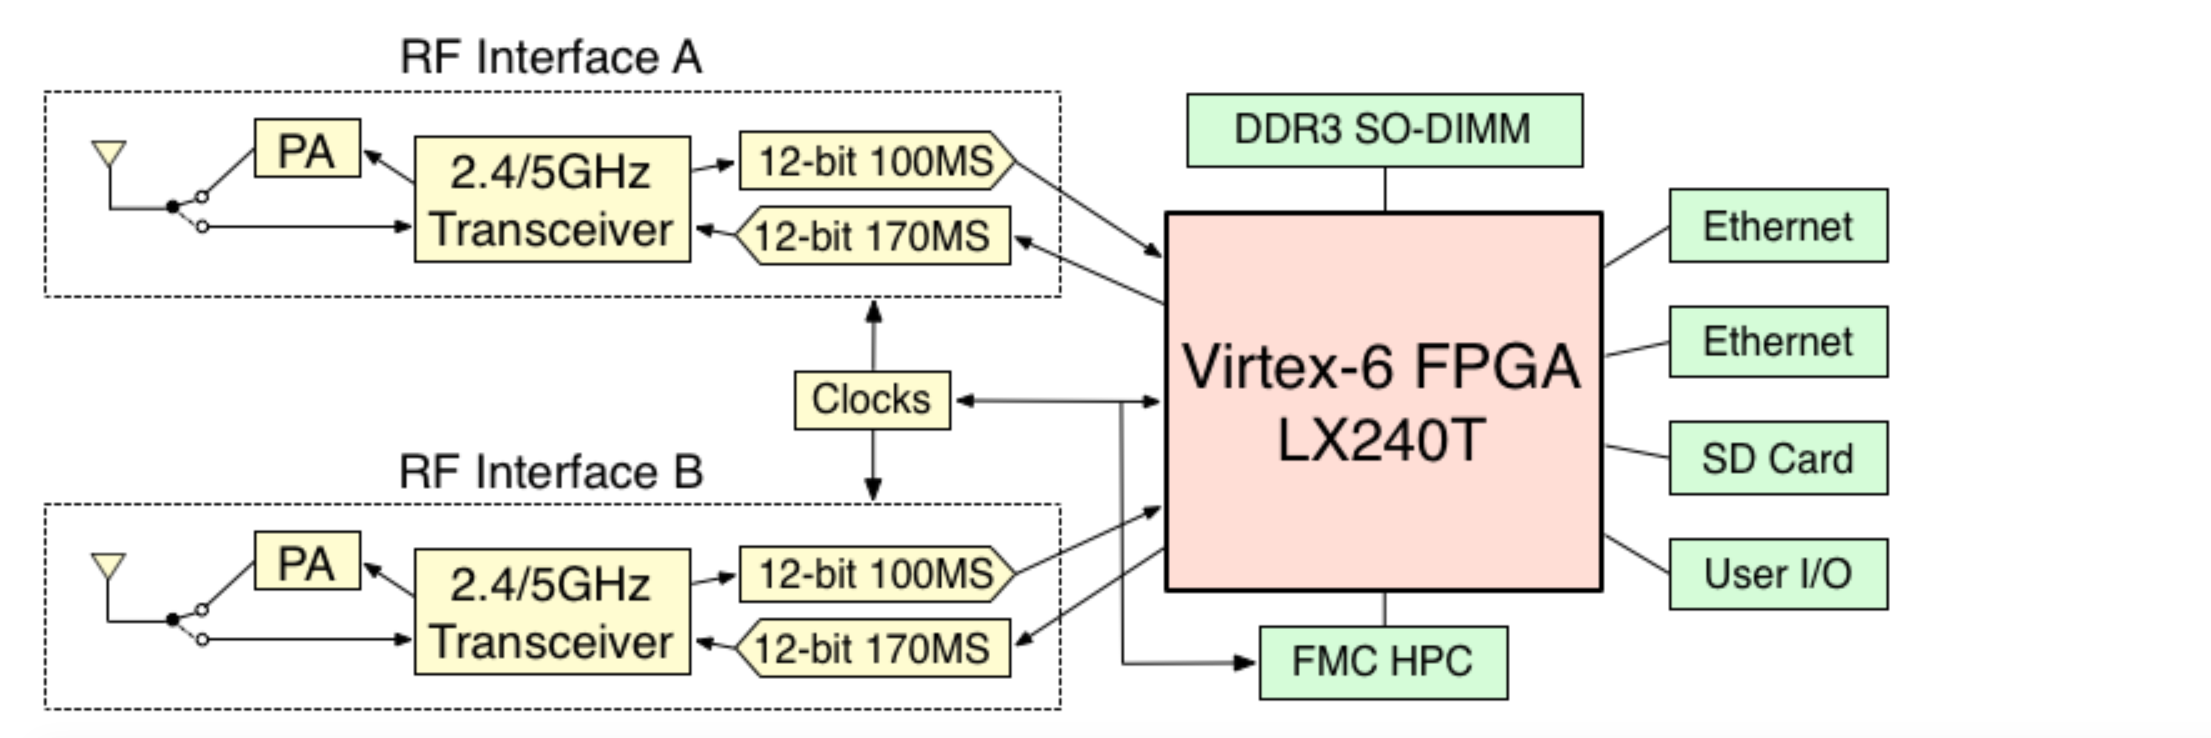
\includegraphics[width = 16cm,height=6cm]{RF-inteface.png}
\caption{Design des Warp v3 Kits  \cite{[3]}}
\label{fig3}
\end{center}
\end{figure}
\noindent Die RF Interfaces verfügen jeweils über einen 12 Bit Digital Analog Wandler mit maximal 100 Mega Samples pro Sekunde, einen 12 Bit Analog Digital Wandler mit maximal 170 Mega Samples pro Sekunde, einen Transceiver, der sowohl 2,4 GHz als auch 5GHz implementiert, einen Dual Band Verstärker für den Sendepfad sowie einen Switch, um zwischen Sende- und Empfangspfad zu wechseln. Den Abschluss jedes RF Interfaces bildet ein Koaxialer Stecker für Hochfrequenzanwendungen (SMA).\\
\\
\noindent \textbf{Taktfrequenz}\\
Das Mango v3 Kit verfügt über 2 unabhängige  Oszillatoren. Einen mit einer Taktfrequenz von 200 MHz für das FPGA und einen eigenen für die RF Interfaces, die beide auf den selben Oszillator zugreifen, mit einer Taktfrequenz von 80 MHz, was dem Basisband entspricht. Es können auch eigene Taktfrequenzen über den FMC Slot eingefügt werden. Das Einstellen der Taktfrequenz im FPGA und den RF Interfaces mit den Oszillatorfrequenzen ist nicht ganz einfach und erfordert einiges Wissen über die Bauteile und macht das Einstellen der Taktfrequenz so hinreichend komplex. Die beiden Puffer Bausteine in \autoref{fig4} geben die jeweilige Taktfrequenz an das RF Interface weiter, wobei der Sampling Clock Buffer noch über einen Teiler verfügt.
\begin{figure}[H]
\begin{center}
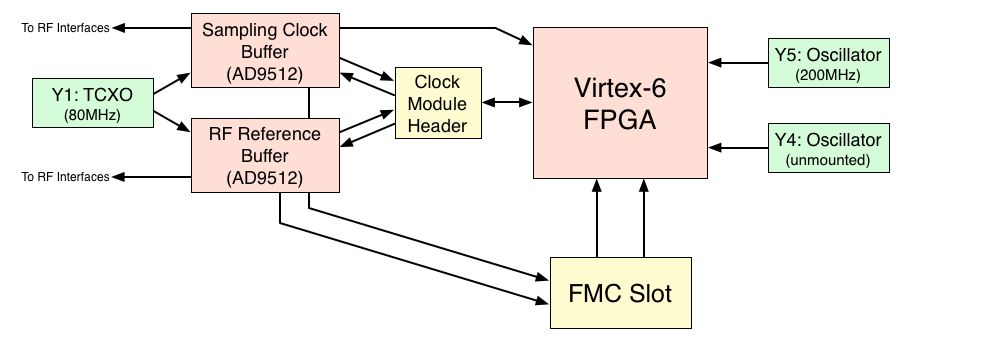
\includegraphics[width = 16cm,height=6cm]{Unbenannt.jpg}
\caption{Übersicht über die Taktung des Mango v3 Kits \cite{[4]}}
\label{fig4}
\end{center}
\end{figure}
\noindent\textbf{Einstellen des Analog/Digital- und Digital/Analogwandlers}\\
Der erste Baustein jedes RF Interfaces ist das
10/12-Bit Schwachstrom Breitband Mixed Signal Front End(MxFE) AD9963, dieser Baustein beinhaltet sowohl den Analog/Digitalwandler (ADC) als auch den Digital/Analogwandler (DAC). Der DAC verfügt über einen 3 stufigen Interpolationsfilter, der eine 1x-,2x-,4x- oder 8x-fache Abtastratenerhöhung ermöglicht. Die Interpolationsstufen können zur Laufzeit über ein SPI-Interface eingestellt werden in dem folgende Registerflags aus \autoref{tab:tabelle1} gesetzt werden.
\begin{figure}[H]
\begin{center}
\begin{tabular}{|c|c|p{7cm}}\hline
\small
  \textbf{Interpolationsstufe} & \textbf{DAC Registerflags} \\ \hline
  1x & - \\\hline
  2x & INT0\\\hline
  4x & INT0, INT1 \\\hline
  8x & INT0, INT1 \\\hline
 \end{tabular}
 \caption{Zu setzende Register für die Auswahl des Interpolationsfilters}
  \label{tab:tabelle1}
  \end{center}
 \end{figure}
\noindent Der ADC verfügt über einen 2x-fachen Dezimator der durch das Registerflag "DEC" zur Laufzeit über SPI ein- bzw. ausgeschaltet werden kann.
Um die richtige, gewünschte Abtastfrequenz für den DAC und ADC einzustellen muss sowohl der Takt der TXCLK vom FPGA, die Taktausgabe des Refernce Buffers, der Divider des Sampling Clock Buffers als auch der Devider bzw. Interpolationsfilter richtig eingestellt werden.\\
\\
\noindent\textbf{Transceiver, Verstärker und Switch  }\\
Hinter dem AD9963 sitzt der MAX2829 Transceiver, dieser generiert das Trägersignal und kann sowohl 2,4GHz als auch den 5GHz Bereich implementieren. Nach dem Transceiver folgt der Verstärker oder Power Amplifier (PA) und der Switch der zwischen Sende- und Empfangspfad wählt. Alle drei Bausteine können über SPI eingestellt werden.

\section{Das Warp Reference Design 802.11}
\label{sc:802.11rd}
\small Author: Philipp Sebastian Schmieder\\
\Large
Das Einstellen des RF Interfaces stellt alleine durch das abstimmen der Taktfrequenzen eine relativ komplexe Aufgabe dar, dabei hat man sich noch nicht mit dem Design für das FPGA beschäftigt, welches wahrscheinlich noch einmal mehrere Monate Zeit kostet. Um ein grundlegendes Design für das FPGA und das RF Interface zu haben, gibt es von der Warp Website ein Referenz Design für diverse IEEE 802.11 Standards. Das Referenz Design implementiert jeweilige OFDM PHYs und DCF MACs und enthält fertige Designs für  802.11a, 802.11g und 802.11n. Es macht Sinn für die Grundeinstellung auf das Referenz Design zuzugreifen da man so eine Echtzeit FPGA Implementierung bekommt und einen ersten Ansatzpunkt hat um den PHY und MAC des IEEE 802.11p-Standard auf dem Mango v3 Kit zu implementieren.
\begin{figure}[H]
\begin{center}
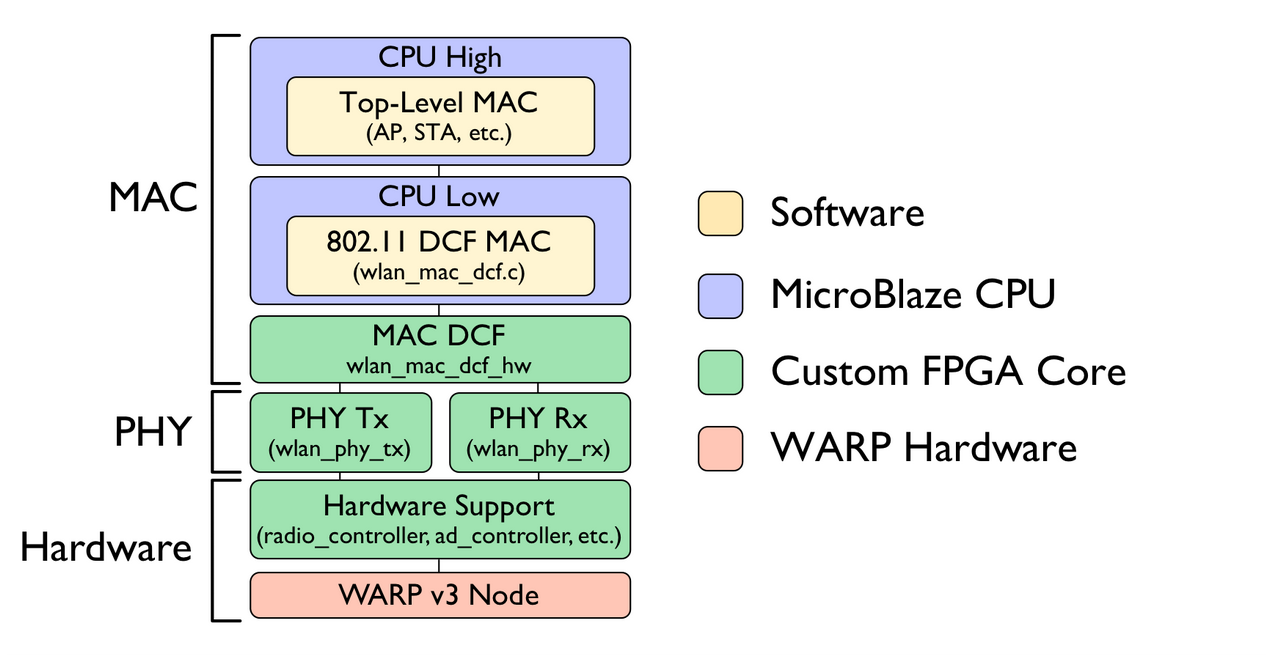
\includegraphics[width = 16cm,height=10cm]{Archreferencedesign.png}
\caption{Aufbau des Warp 802.11 Reference Designs  \cite{[5]}}
\label{fig5}
\end{center}
\end{figure}
\noindent \autoref{fig5} gibt einen Überblick über die Kerne des Referenz Design und zeigt wo diese hinterlegt sind. Die beiden CPU Kerne, CPU High und CPU Low, sind auf 2 Micro Blaze CPUs implementiert. Die Micro Blaze CPU ist ein von Xilinx entworfenes Design um CPUs auf dem FPGA zu konfigurieren, dem entsprechend laufen die beiden CPUs in einem Design im FPGA des Mango v3 Kit. CPU High übernimmt unter anderem das Senden aller Pakete die nicht zum Kontrollfluss gehören, er kontrolliert alle Handshakes mit anderen Knoten und falls Daten über die Ethernetschnittstelle weitergeleitet oder von dieser über das RF Interface gesendet werden sollen, übernimmt dieser Kern das ein- bzw. auspacken.
Die CPU Low übernimmt alle Interaktionen zwischen dem MAC und dem PHY, sowie das senden von ACKs, planen von Backoffs, einstellen des Contention Windows und initiiert erneute Übertragungen falls nötig.
Der MAC DCF ist direkt auf dem FPGA implementiert und ist die Schnittstelle der beiden PHY Kerne Tx und Rx zur MAC Schicht. In diesem Kern sind unter anderem die Carrier Sense Mechanismen und die Taktzyklen realisiert.
In den PHY Tx und PHY Rx Kernen befindet sich die Implementierungen der physikalischen OFDM Schicht, hier werden Daten umgewandelt und in Signale verpackt bzw. Signale ausgepackt und in Daten gewandelt. In dem letzten Kern, dem Hardware Support, liegen alle Treiber für das Kit.
Um genau zu verstehen wie das Referenz Design einen Standard implementiert, lohnt es sich die Umsetzung des 802.11a Standard genauer anzusehen und zu versuchen 2 verschiedenen Warp v3 Kits miteinander kommunizieren zu lassen. Ist der Schritt gelungen kann 802.11a so angepasst werden, dass der PHY und MAC zum 802.11p passen.
\section{IEEE Standard 802.11p}
\label{802.11p}
\small Author: Philipp Sebastian Schmieder\\
\Large
Um zu verstehen was man beim 802.11a-Standard ändern muss um den 802.11p-Standard nachzubilden, müssen zunächst die Unterschiede zwischen diesen beiden Standards geklärt werden. Hier soll nun der 802.11p-Standard und dessen Aufbau im PHY und MAC erklärt werden.
\subsection{Der PHY Layer}
Zunächst ist es wichtig zu verstehen wie der PHY bei 802.11p aufgebaut ist, also wie die Kanäle, das Frequenzband und die Modulation aussehen.
Das Frequenzband und die Kanäle von 802.11p liegen im 5GHz Bereich. \autoref{tab:tabelle2} gibt einen Überblick über alle Frequenzen und Kanäle, der Kanaltyp ist als CCH oder SCH angegeben. CCH ist Kontrollkanal für Signalisierungs- und Steuerungsinformationen und SCH sind Synchronisationskanäle und dienen z.B. zur Erkennung der Kanalstruktur.
\begin{figure}[H]
\begin{center}
\begin{tabular}{|c|c|c|}\hline
\small
  \textbf{Kanaltyp} & \textbf{Mittenfrequenz}  & \textbf{Kanalnummer} \\ \hline
  G5-CCH & 5,9 GHz & 180 \\\hline
  G5-SCH1 & 5,880 GHz & 176 \\\hline
  G5-SCH2 & 5,890 GHz & 178 \\\hline
  G5-SCH3 & 5,870 GHz & 174 \\\hline
  G5-SCH4 & 5,860 GHz & 172 \\\hline
  G5-SCH5 & 5,910 GHz & 182 \\\hline
  G5-SCH6 & 5,920 GHz & 184 \\\hline
 \end{tabular}
 \caption{Frequenzen und Kanäle für IEEE 802.11p nach  \cite{etsi}}
  \label{tab:tabelle2}
  \end{center}
 \end{figure}
\noindent Im Gegensatz zu 802.11a liegt bei 802.11p die \textbf{Bandbreite bei 10MHz}, das Modulationsverfahren ist \textbf{OFDM mit 52 Subcarriern} (48 Data Carriers und 4 Pilot Carriers). Die Modulationsarten sind equivalent zu 802.11a.
\cite{etsi}
\subsection{Der MAC Layer}
Der Kanalzugriff im MAC Layer erfolgt Ad-hoc, das heißt es gibt keinen einzelnen Access Point und die Teilnehmer konkurrieren um die Kanäle. Die Kollisionskontrolle erfolgt durch Carrier Sense Mutiple Access / Collision Avoidence(CSMA/CA). Der Quality of Service wird durch das prioritätsbasierte Verfahren Enhanced Distributed Channel Access realisiert (EDCA).

\small
\normalsize

\newpage
\section{Umsetzung}\label{umsetzung}
\small Author: Dominik Bayerl\\
\Large

Im Rahmen des Projekts wurden die zwei grundsätzlichen Funktionen
umgesetzt, die zur Nutzung der Hardware für weitere Experimente
erforderlich sind. Dies ist einerseits die Erweiterung des
802.11-Reference-Designs auf den 802.11p-Standard und andererseits die
Implementierung einer Ethernet-Schnittstelle zum Empfang und Senden von
Daten über einen angeschlossenen Computer. Auf beide Funktionen soll im
Folgenden kurz eingegangen werden.

\subsection{WARP Reference Design für
802.11p}\label{warp-reference-design-fuxfcr-802.11p}

Auf die grundsätzliche Funktionsweise von \emph{802.11p} wurde bereits
in \cref{802.11p} eingegangen. Dabei wurde deutlich,
dass der Standard sehr ähnlich zum bereits implementierten
\emph{802.11a} ist (insbesondere die \ac{ofdm}-Waveform) und sich vor
allem in zwei wesentlichen Merkmalen, den Channel-Frequenzen und der
Channel-Bandbreite unterscheidet. Es bietet sich daher an, die
Implementierung auf Basis des vorhandenen Frameworks vorzunehmen.

\subsubsection{Channel-Frequenzen}\label{channel-frequenzen}

Für das Teilnehmer-Multiplexing in WLAN-Funksystemen werden
üblicherweise Channels verwendet, d.h. es können mehrere getrennte
Funknetze dadurch unabhängig voneinander existieren, indem sie
verschiedene Channels und dadurch verschiedene Frequenzen für die
Kommunikation nutzen. Im 802.11p Standard sind acht verschiedene
Channel-Typen spezifiziert, die für unterschiedliche Aufgaben reserviert
sind. \Cref{tbl:channels} gibt einen Überblick über die
spezifizierten Kanäle \autocite{etsi}.

\begin{longtable}[]{@{}lllll@{}}
\caption{802.11p Channels.}\label{tbl:channels}\tabularnewline
\toprule
\begin{minipage}[b]{0.08\columnwidth}\raggedright\strut
Channel Type\strut
\end{minipage} & \begin{minipage}[b]{0.30\columnwidth}\raggedright\strut
Center frequency\strut
\end{minipage} & \begin{minipage}[b]{0.16\columnwidth}\raggedright\strut
IEEE 802.11 channel number\strut
\end{minipage} & \begin{minipage}[b]{0.14\columnwidth}\raggedright\strut
Channel spacing\strut
\end{minipage} & \begin{minipage}[b]{0.18\columnwidth}\raggedright\strut
Default data rate\strut
\end{minipage}\tabularnewline
\midrule
\endfirsthead
\toprule
\begin{minipage}[b]{0.08\columnwidth}\raggedright\strut
Channel Type\strut
\end{minipage} & \begin{minipage}[b]{0.30\columnwidth}\raggedright\strut
Center frequency\strut
\end{minipage} & \begin{minipage}[b]{0.16\columnwidth}\raggedright\strut
IEEE 802.11 channel number\strut
\end{minipage} & \begin{minipage}[b]{0.14\columnwidth}\raggedright\strut
Channel spacing\strut
\end{minipage} & \begin{minipage}[b]{0.18\columnwidth}\raggedright\strut
Default data rate\strut
\end{minipage}\tabularnewline
\midrule
\endhead
\begin{minipage}[t]{0.08\columnwidth}\raggedright\strut
G5-CCH\strut
\end{minipage} & \begin{minipage}[t]{0.30\columnwidth}\raggedright\strut
\(\SI{5900}{\mega\hertz}\)\strut
\end{minipage} & \begin{minipage}[t]{0.16\columnwidth}\raggedright\strut
180\strut
\end{minipage} & \begin{minipage}[t]{0.14\columnwidth}\raggedright\strut
\(\SI{10}{\mega\hertz}\)\strut
\end{minipage} & \begin{minipage}[t]{0.18\columnwidth}\raggedright\strut
\(\SI{6}{Mbps}\)\strut
\end{minipage}\tabularnewline
\begin{minipage}[t]{0.08\columnwidth}\raggedright\strut
G5-SCH2\strut
\end{minipage} & \begin{minipage}[t]{0.30\columnwidth}\raggedright\strut
\(\SI{5890}{\mega\hertz}\)\strut
\end{minipage} & \begin{minipage}[t]{0.16\columnwidth}\raggedright\strut
178\strut
\end{minipage} & \begin{minipage}[t]{0.14\columnwidth}\raggedright\strut
\(\SI{10}{\mega\hertz}\)\strut
\end{minipage} & \begin{minipage}[t]{0.18\columnwidth}\raggedright\strut
\(\SI{12}{Mbps}\)\strut
\end{minipage}\tabularnewline
\begin{minipage}[t]{0.08\columnwidth}\raggedright\strut
G5-SCH1\strut
\end{minipage} & \begin{minipage}[t]{0.30\columnwidth}\raggedright\strut
\(\SI{5880}{\mega\hertz}\)\strut
\end{minipage} & \begin{minipage}[t]{0.16\columnwidth}\raggedright\strut
176\strut
\end{minipage} & \begin{minipage}[t]{0.14\columnwidth}\raggedright\strut
\(\SI{10}{\mega\hertz}\)\strut
\end{minipage} & \begin{minipage}[t]{0.18\columnwidth}\raggedright\strut
\(\SI{6}{Mbps}\)\strut
\end{minipage}\tabularnewline
\begin{minipage}[t]{0.08\columnwidth}\raggedright\strut
G5-SCH3\strut
\end{minipage} & \begin{minipage}[t]{0.30\columnwidth}\raggedright\strut
\(\SI{5870}{\mega\hertz}\)\strut
\end{minipage} & \begin{minipage}[t]{0.16\columnwidth}\raggedright\strut
174\strut
\end{minipage} & \begin{minipage}[t]{0.14\columnwidth}\raggedright\strut
\(\SI{10}{\mega\hertz}\)\strut
\end{minipage} & \begin{minipage}[t]{0.18\columnwidth}\raggedright\strut
\(\SI{6}{Mbps}\)\strut
\end{minipage}\tabularnewline
\begin{minipage}[t]{0.08\columnwidth}\raggedright\strut
G5-SCH4\strut
\end{minipage} & \begin{minipage}[t]{0.30\columnwidth}\raggedright\strut
\(\SI{5860}{\mega\hertz}\)\strut
\end{minipage} & \begin{minipage}[t]{0.16\columnwidth}\raggedright\strut
172\strut
\end{minipage} & \begin{minipage}[t]{0.14\columnwidth}\raggedright\strut
\(\SI{10}{\mega\hertz}\)\strut
\end{minipage} & \begin{minipage}[t]{0.18\columnwidth}\raggedright\strut
\(\SI{6}{Mbps}\)\strut
\end{minipage}\tabularnewline
\begin{minipage}[t]{0.08\columnwidth}\raggedright\strut
G5-SCH5\strut
\end{minipage} & \begin{minipage}[t]{0.30\columnwidth}\raggedright\strut
\(\SI{5850}{\mega\hertz}\)\strut
\end{minipage} & \begin{minipage}[t]{0.16\columnwidth}\raggedright\strut
182\strut
\end{minipage} & \begin{minipage}[t]{0.14\columnwidth}\raggedright\strut
\(\SI{10}{\mega\hertz}\)\strut
\end{minipage} & \begin{minipage}[t]{0.18\columnwidth}\raggedright\strut
\(\SI{6}{Mbps}\)\strut
\end{minipage}\tabularnewline
\begin{minipage}[t]{0.08\columnwidth}\raggedright\strut
G5-SCH6\strut
\end{minipage} & \begin{minipage}[t]{0.30\columnwidth}\raggedright\strut
\(\SI{5910}{\mega\hertz}\)\strut
\end{minipage} & \begin{minipage}[t]{0.16\columnwidth}\raggedright\strut
184\strut
\end{minipage} & \begin{minipage}[t]{0.14\columnwidth}\raggedright\strut
\(\SI{10}{\mega\hertz}\)\strut
\end{minipage} & \begin{minipage}[t]{0.18\columnwidth}\raggedright\strut
\(\SI{6}{Mbps}\)\strut
\end{minipage}\tabularnewline
\begin{minipage}[t]{0.08\columnwidth}\raggedright\strut
G5-SCH7\strut
\end{minipage} & \begin{minipage}[t]{0.30\columnwidth}\raggedright\strut
nach IEEE 802.11, \(\SIrange{5470}{5725}{\mega\hertz}\)\strut
\end{minipage} & \begin{minipage}[t]{0.16\columnwidth}\raggedright\strut
94 bis 145\strut
\end{minipage} & \begin{minipage}[t]{0.14\columnwidth}\raggedright\strut
verschiedene\strut
\end{minipage} & \begin{minipage}[t]{0.18\columnwidth}\raggedright\strut
abhängig von der Bandbreite\strut
\end{minipage}\tabularnewline
\bottomrule
\end{longtable}

Es wird deutlich, dass eine Erweiterung des verfügbaren Frequenzbandes
von 802.11a (\(\SIrange{5180}{5825}{\mega\hertz}\)) auf 802.11p
(\(\SIrange{5850}{5925}{\mega\hertz}\)) notwendig ist.

Die \ac{rf}-Frequenz wird auf dem Mango WARPv3 Board durch den
\ac{rf}-Transceiver MAX2829 (siehe \cref{sec:hardware})
erzeugt. Dieser kann via \ac{spi} durch die Low-CPU des \ac{fpga}
konfiguriert werden \autocite{max2829}. Zur Einstellung der
Center-Frequenz des Transceivers sind dabei insbesondere die Register
\emph{Band Select and PLL}, \emph{Integer-Divider Ratio} und
\emph{Fractional-Divider Ratio} wichtig. Über das \emph{Band Select}
Register wird das Frequenzband (\(\SI{5}{\giga\hertz}\)) ausgewählt und
durch den Vorteiler (engl. Divider) wird die Grundfrequenz des
Oszillators durch einen rationalen Teiler (Ganzzahl und Fraktion) auf
den gewünschten Wert abgeleitet. Zur Anpassung der verfügbaren
Frequenzen ist daher eine Änderung der möglichen Register-Werte des
\ac{rf}-Transceivers notwendig.

Im WARP Reference Design erfolgt die Konfiguration des Transceivers
durch den radio\_controller IP Core. Änderungen der Konfiguration
erfolgen also am elegantesten im Treiber des Peripherals. Konkret
bedeutet dies, dass in der Datei \path{edk/pcores/radio_controller.c}
Änderungen für drei Lookup-Tables
\texttt{rc\_tuningParams\_5GHz\_freqs},
\texttt{rc\_tuningParams\_5GHz\_reg3} und
\texttt{rc\_tuningParams\_5GHz\_reg4} notwendig sind, nämlich müssen die
Register-Werte für die hinzugefügten Channels hinterlegt werden. Die
Berechnung der Werte kann händisch nach \autocite{max2829} oder durch
das beiligende Python-Skript erfolgen.

Anschließend müssen die zusätzlichen Kanäle zur Verwendung
``freigeschalten'' werden. Dies erfolgt in der Software der Low-CPU.

\subsubsection{Channel Bandbreite}\label{channel-bandbreite}

Die verwendete Bandbreite des Kanals hängt direkt von der gewählten
Sampling-Rate des verwendeten \ac{adc}/\ac{dac}-Wandlers AD9963 ab.
Dieser ist ebenfalls über die \ac{spi}-Schnittstelle durch die Low-CPU
konfigurierbar, die Implementierung erfolgt über den w3\_ad\_controller
Core.

Für 802.11p werden vorrangig Kanäle der Bandbreite
\(\SI{10}{\mega\hertz}\) verwendet. Diese Bandbreite ist bereits im
802.11 Reference Design implementiert, muss jedoch in der Software der
Low-CPU durch einen Aufruf der Funktion \texttt{set\_phy\_samp\_rate()}
aktiviert werden. Der \(\SI{10}{\mega\hertz}\)-Modus wird dabei durch
die Konstante \texttt{PHY\_10M} ausgewählt.

Im 802.11p Reference Design wird ist dies im
\emph{wlan\_mac\_low\_11p}-Projekt implementiert.

\subsection{Validierung der Umsetzung am Spektrometer}
Eine Möglichkeit die Implementierung auf der Plattform zur Validierung war die Auswertung des Ausgangssignals an einem Spektrometer. Zunächst wurde das Signal bei Einstellen des 802.11a-Standards gemessen.
\begin{figure}[H]
\begin{center}
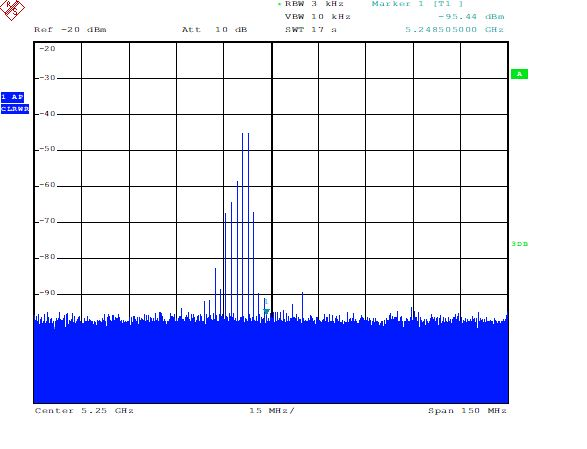
\includegraphics[width = 16cm,height=10cm]{80211a.jpg}
\caption{Signal des Warp V3 Boards mit 802.11a}
\label{fig6}
\end{center}
\end{figure}
\noindent In der Auswertung ist gut zu erkennen, dass das Kit die eingestellte Centerfrequenz bei 5,2GHz genau  trifft und auch die Bandbreite mit 20MHz passt. Als nächstes wurde das Mango v3 Kit auf den 802.11p-Standard eingestellt und das Ausgangssignal vermessen. Auch hier wird die eingestellte Centerfrequenz bei 5,9 GHz getroffen und auch die Bandbreite stimmt mit 10MHz. Somit konnte verifiziert werden, dass die Plattform den 802.11p PHY implementiert und das Mango v3 Kit standardkonform sendet.
\begin{figure}[H]
\begin{center}
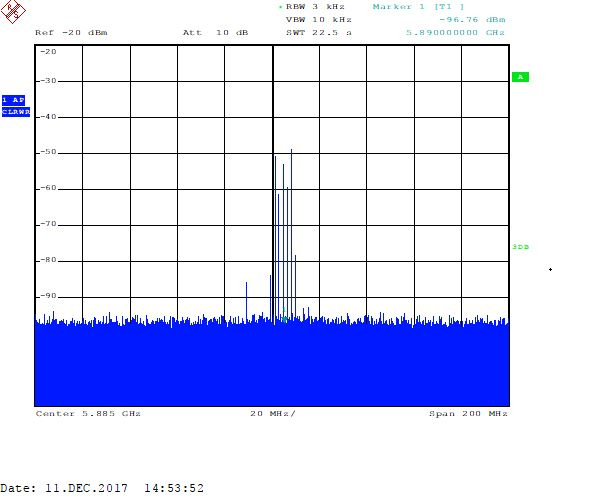
\includegraphics[width = 16cm,height=10cm]{80211p.jpg}
\caption{Signal des Warp v3 Boards mit 802.11p}
\label{fig7}
\end{center}
\end{figure}


\subsection{Ethernet-Schnittstelle}\label{ethernet-schnittstelle}

Für das Projekt wurde beschlossen, dass die Umsetzung von Funktionalität
möglichst auf einem normalen Computer erfolgen soll. Die Gründe dafür
sind, dass dort bereits eine Vielzahl von spezialisierten Tools (u.a.
Wireshark und PCAP) vorhanden sind, deren Implementierung den Rahmen des
Projekts bei weitem sprengen würde. Zusätzlich ermöglicht wird es
dadurch einfacher ermöglicht, Fehler in der Software zu debuggen und
3rd-party Komponenten (wie beispielsweise MATLAB) anzubinden.

Die Realisierung dieser Design-Ziele erfolgt durch die Instrumentierung
des WARP v3 Board über eome Ethernet-Schnittstelle. Darüber können
sowohl Daten des WLAN-Kanals empfangen und an einen Computer
weitergeleitet, als auch Daten von einem normalen Rechner als 802.11p
Frames gesendet werden.

\subsubsection{Hardware}\label{hardware}

Das WARPv3 Board besitzt zwei \(\SI{1}{Gbps}\)-Ethernet-Interfaces.
Dabei ist Interface \textbf{B} durch das Reference-Design reserviert, um
darüber Experimente steuern zu können\autocite{warp-exp}. Die
Schnittstelle zur Datenübertragung wurde deshalb auf Interface
\textbf{A} realisiert. Diese kann über ein normales RJ45 Ethernet-Kabel
mit einem beliebigen Rechner verbunden werden.

\subsubsection{RFtap}\label{rftap}

Die Übertragung der WLAN-Frames über eine Ethernet-Schnittstelle ist nur
möglich, wenn diese vorher in ein entsprechendes Transport-Protokoll
verpackt werden. Dies ist dem Umstand geschuldet, dass 802.11-Frames
keine gültigen Ethernet(-II)-Frames sind und umgekehrt. Würde das
WARP-Board die empfangenen 802.11 Frames vollständig identisch auf die
Ethernet-Schnittstelle übertragen, werden die Frames von der
Netzwerkkarte des angeschlossenen Rechners verworfen und erreichen
dessen Betriebssystem bzw. Anwendungen erst gar nicht.

Es wurden zwei verschiedene Protokolle zur Übertragung von 802.11 Frames
über die Ethernet-Schnittstelle evaluiert: - radiotap, das spezialisiert
ist auf ``{[}\ldots{}{]} 802.11 frame injection and
reception''\autocite{radiotap} - RFtap, ein Protokoll ``{[}\ldots{}{]}
designed to provide Radio Frequency (RF) metadata about
packets''\autocite{rftap}

Für beide Protokolle existiert eine gute Unterstützung in bestehenden
Netzwerk-Analyse Tools wie Wireshark. Im Rahmen des Projekts wurde das
\emph{RFtap} Protokoll in die High-CPU Software implementiert. Die
Gründe dafür sind die einfachere Implementierung gegenüber radiotap und
die erweiterte Funktionalität. Da ein RFtap-Frame verschiedenste
Payload-Pakete verpacken kann, ist es unter anderem auch möglich, damit
radiotap-Frames zu übertragen. RFtap kann folglich als Obermenge von
radiotap angesehen werden. Zusätzlich ist es mit RFtap Möglich, die
empfangenen Pakete um weitere Informationen (insbesondere physikalische
Parameter) zu annotieren. \Cref{fig:rftap} zeigt
schematisch den Aufbau eines RFtap-Frames.

\begin{figure}
\centering
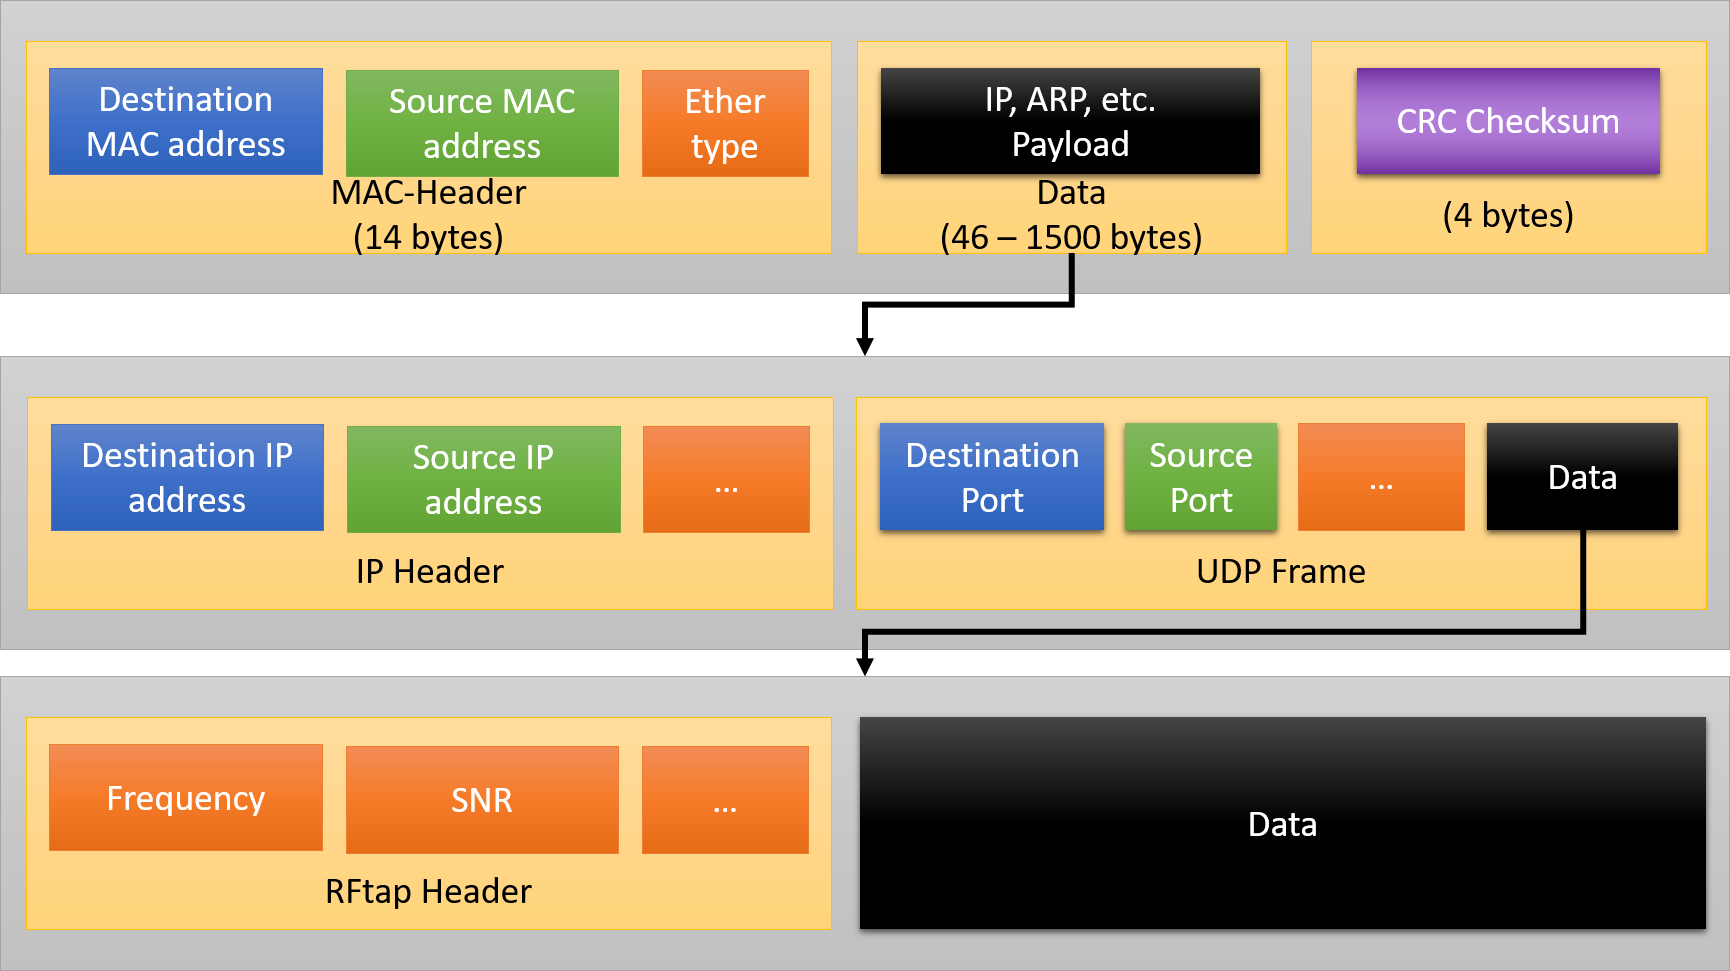
\includegraphics[width=0.8\textwidth]{rftap.png}
\caption{RFtap Frame Aufbau.}\label{fig:rftap}
\end{figure}

Für die direkte Verbindung zwischen dem WARPv3 Board und einem Computer
sind die verwendeten MAC- und IP-Adressen unkritisch, da auf den
Interfaces in diesem Fall keine Filterung stattfindet. In der
derzeitigen Implementierung sind die Felder daher leer (Wert 0). Für
künftige Projekte wäre es denkbar, diese Informationen sinnvoll zu
befüllen. Dies ermöglicht beispielsweise ein Routing von RFtap-Frames
über gewöhnliche, kommerzielle Netzwerk-Hardware.

In Wireshark sind RFtap-Dissectors für UDP-Frames auf Destination-Port
\textbf{52001} implementiert. Erkannt werden die Frames durch die Magic
Numbers \texttt{0x52\ 0x46\ 0x74\ 0x61} (ascii: RFta) zu Beginn des
Frames. Es folgt die Länge (unsigned integer, 2 Byte) des RFtap-Headers
(ohne Datenteil!) in 32-bit Words und ein Flags-Bitfield (2 Byte), das
die nachfolgenden Header-Flags
spezifiziert\autocite{rftap-specifications}. Dabei können (aufgrund des
Längenfelds) beliebige zusätzliche Felder an das Ende des Headers
angefügt werden, die dann jedoch nicht durch einen Dissector abgedeckt
werden können. Der RFtap-Frame endet mit dem RF-Payload. Besonders
interessant ist die Angabe des \ac{dlt}-Felds, da dadurch der Typ der
Nutzdaten spezifiziert wird. Bei korrekter Angabe nutzt Wireshark dann
automatisch den richtigen Dissector um die Payload zu analysieren
(beispielsweise LINKTYPE\_IEEE802\_11, IEEE 802.11 wireless LAN Frame
\autocite{tcpdump}).

Das Senden von Frames von einem Rechner erfolgt analog, in umgekehrter
Reihenfolge.


\section{Optimierungsmöglichkeiten und weitere
Ideen}\label{optimierungsmuxf6glichkeiten-und-weitere-ideen}
\small Author: Dominik Bayerl\\
\Large

Zum derzeitigen Zeitpunkt bestehen noch offene Punkte zur weiteren
Optimierung der Software, die aufgrund des beschränkten zeitlichen
Rahmes des Projektes nicht mehr umgesetzt werden konnten.

Dabei handelt es sich größtenteils um Unschönheiten und
Performance-Maßnahmen in der Software der High-CPU
(Sniffer-Applikation), die jedoch nicht die grundsätzliche Funktion
einschränken. Einige Verbesserungen sollen im Folgenden knapp skizziert
werden.

\subsection{Optimierung des IP-Stacks}
\label{optimierung-des-ip-stacks}

Der IP-Stack wird immer dann benötigt, wenn ein Paket vom Wireless auf
das LAN-Interface übertragen wird und umgekehrt. Beispielsweise ist es
zur Verpackung der WLAN-Frames notwendig, diese in das RFtap-Format zu
bringen, wobei dieses aus einem UDP-Frame besteht. Derzeit ist dies in
der Datei \path{wlan_mac_high_sniffer/rftap.c} als
Chainable-Funktionen implementiert. Dies bedeutet, dass die einzelnen
Bestandteile des Ethernet-Frames stückweise konstruiert und dem Buffer
hinzugefügt werden. Dadurch, dass der Buffer front-alloziert ist (d.h.
es ist lediglich die Start-Adresse und die Länge des Buffers bekannt)
ist es nicht möglich, die Header der Frames direkt dem Beginn des
Buffers hinzuzufügen, da andernfalls der Datenbereich des Frames
überschrieben werden würde. Um dies zu umgehen werden alle Header in
einem separaten Buffer abgelegt und anschließend der Datenteil an das
Ende der Header kopiert (Funktion \texttt{mpdu\_rx\_process()} in
\path{wlan_mac_high_sniffer/wlan_mac_sniffer.c}). Der
Kopiervorgang ist dabei potentiell ein Performance-Flaschenhals. Die
Notwendigkeit eines einzelnen Buffers der den kompletten Ethernet-Frame
enthält, ergibt sich durch die derzeitige Verwendung des
Ethernet-Interfaces des \ac{fpga} im einfachen \ac{dma}-Modus. Die
tatsächliche Übertragung der Daten auf die Ethernet-Schnittstelle
erfolgt anschließend ohne weitere Beteiligung der CPU durch das
Ethernet-Peripheral.

Im erweiterten \ac{dma}-Modus bietet der Ethernet-\ac{ip-core} die
Möglichkeit der Datenübertragung zur Ethernet-Schnittstelle aus
verschiedenen Speicherbereichen. Dieses Konzept wird bei Xilinx als
``Scatter-Gather-\ac{dma}'' (\emph{grobe Übersetzung}:
Verstreutes-Sammeln-\ac{dma}) bezeichnet
\autocite{xilinx-ethernet-core}. Die Funktionsweise besteht darin, dass
der \ac{dma}-Schnittstelle nicht mehr die Buffer-Adresse und deren Länge
übergeben wird, sondern die Adresse eines sogenannten ``Buffer
Descriptors''. Diese Datenstruktur besteht unter anderem aus der
Buffer-Adresse und einem Längenfeld (siehe \cref{fig:dma}).
Sobald das \ac{dma}-Peripheral alle Daten aus dem im Buffer Descriptor
referenzierten Buffers übertragen hat, wird ein Interrupt an die CPU ausgelöst.

\begin{figure}
\centering
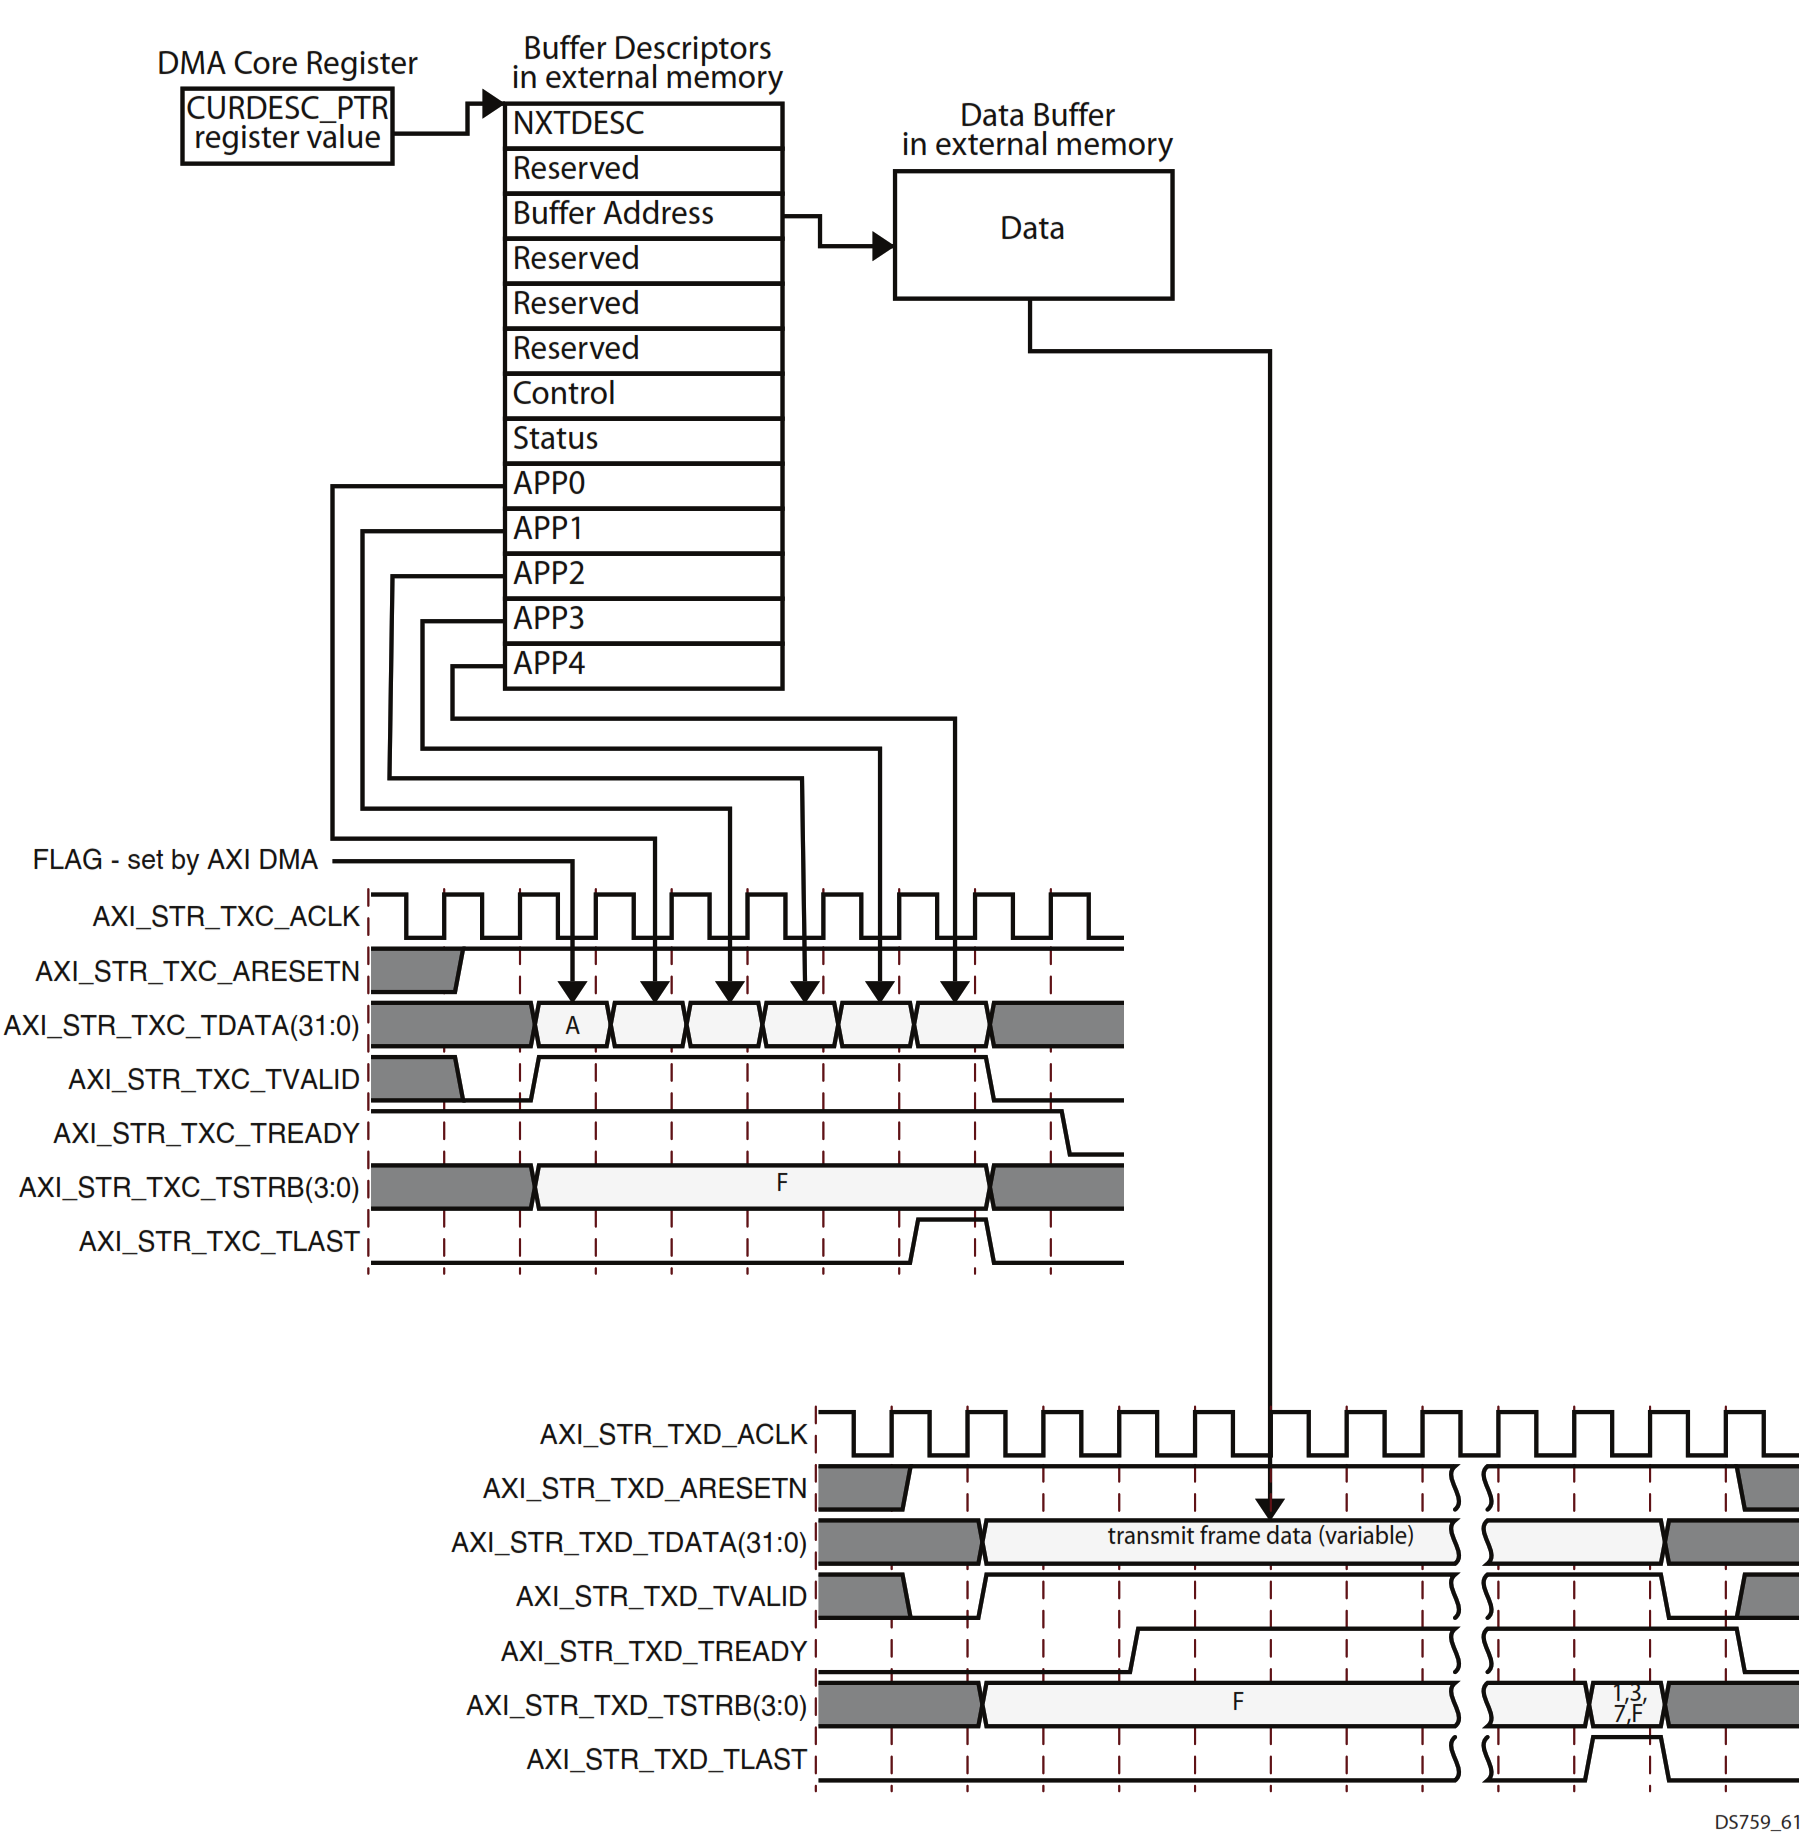
\includegraphics[width=0.8\textwidth]{ds759_axi_ethernet_075.png}
\caption{Xilinx \ac{dma} Buffer Descriptors\autocite{xilinx-ethernet-core}.}
\label{fig:dma}
\end{figure}

Der Vorteil dieses Verfahrens besteht darin, dass eine zweite
Indirektionsschicht eingeführt wird; dadurch ist es nicht mehr
notwendig, dass sämtliche \ac{dma}-Daten sequentiell im Speicher liegen.
Üblicherweise implementiert man dazu eine Single-Linked-List (\ac{fifo}
Queue) aus Buffer-Descriptors, die nach jedem \ac{dma}-Interrupt
weitergeschalten wird. Für den konkreten Fall der Ethernet-Frames
ermöglicht dieses Verfahren, die einzelnen Header-Bestandteile
unabhängig im Speicher ablegen zu können. Dadurch ist ein echter
Zero-Copy Modus - also ohne Daten kopieren zu müssen - möglich.

\subsection{Nutzung der \ac{cfo}-Estimates}
\label{nutzung-der--estimates}

Im Empfangspfad des WARPv3 existiert bereits ein Block zur Korrektur
eventuell vorhandener Frequenzabweichungen der Sender bzw. des
Empfängers (siehe \cref{sc:802.11rd}). Dabei wird
mittels des \ac{lts}-Feldes über mehrere Frames die Frequenz des
empfangenen Signals gegenüber der Center-Frequenz des gewählten Channels
bestimmt und anschließend zur Korrektur der Fourier-Transformation der
einzelnen Carriers genutzt.

In den meisten kommerziellen WiFi-Transceivern wird die Informationen
anschließend verworfen, da sie für die darüberliegende Schicht (Layer 2,
MAC Layer) nicht benötigt wird. Nicht so im WARP Reference Design: die
geschätzte \ac{cfo} wird durch die Low-CPU an die High-CPU in der
Methode \texttt{mpdu\_rx\_process()} in der Datei
\texttt{wlan\_mac\_high\_sniffer/wlan\_mac\_sniffer.c} als Feld
\texttt{cfo\_est} der Struktur \texttt{rx\_frame\_info\_t} übergeben.
Gleichermaßen wird die Information bereits durch die Sniffer-Applikation
in den RFtap-Frames an die Ethernet-Schnittstelle übertragen (\emph{Flag
3, Frequency offset field is present}). Dies ermöglicht die Auswertung
der \ac{cfo}-Estimates beispielsweise im Wireshark eines angeschlossenen
Computers.

Die Information ist besonders deswegen interessant, da sie (unter
anderem) für zwei Anwendungsfälle genutzt werden kann, die im Folgenden
dagelegt werden sollen:

\subsubsection{Doppler-Effekt}
\label{doppler-effekt}

Wie jedes elektromagnetische Signal unterliegen auch die 802.11p-WLAN
Signale dem Doppler-Effekt. Dieser besagt, dass ein Signal der Frequenz
\(f_S\) das von einem Sender \(S\) an einen Empfänger \(B\) derart
übertragen wird, dass Sender und Empfänger eine Relativgeschwindigkeit
\(v_S - v_B = v \neq 0\) besitzen, beim Beobachter eine
Frequenzabweichung
\(f_{B} = \frac{f_{S}}{\gamma} = f_{S} \sqrt{1-\frac{v^2}{c^2}} \approx f_{S} \left(1 - \frac{v^2}{2c^2}\right)\)
erfährt.

Diese Frequenzabweichung muss durch den Empfänger detektiert und
kompensiert werden. Für die Anwendung WLAN wird dies durch die Korrektor
der \ac{cfo} übernommen. Hat ein Empfänger nun Kenntnis über den
statischen \ac{cfo} (bedingt durch ungenaue Oszillatoren) eines Senders,
kann er durch die Messung des aktuellen \ac{cfo} eine dynamische
Frequenzabweichung bestimmen, bei der der Doppler-Effekt eine nicht
unerhebliche Rolle spielt. Für 802.11p bedeutet dies, dass zwei
Fahrzeuge, die miteinander im Funkkontakt stehen, ihre gegenseitige
Relativgeschwindigkeit ohne Zusatzhardware über die WLAN-Schnittstelle
bestimmen könnten. Dies ermöglicht eine Reihe weiterer Funktionen, wie
Notbremsassistenten, Adaptive Tempomaten und ähnliches.

\subsubsection{PHY-Fingerprinting}
\label{phy-fingerprinting}

In einer separaten Teilgruppe des Projektes wurde ein Verfahren zur
Manipulation von Funknetzen, sog. MAC-Spoofing und Evil-Twin-APs
evaluiert. Die Verfahren basieren darauf, dass die Merkmale die zur
Identifikation der Funkteilnehmer verwendet werden, sehr leicht
manipulierbar sind (MAC-Adresse bzw. SSID/BSSID). Für nicht weiter
kryptographisch gesicherte Netzwerke (Offene WLANs) stellen diese
Attacken ein erhebliches Sicherheitsrisiko dar, da dadurch eine Reihe
weiterer Angriffe (Man-in-the-middle, Phishing, ARP-Spoofing, \ldots{})
ermöglicht werden.

Das Mango-Board bietet gegenüber kommerzieller WLAN-Hardware die
Möglichkeit, sämtliche Parameter der Funkübertragung zu erfassen,
insbesondere auch die des physikalischen Layers, beispielsweise in Form
der Center-Frequency-Offsets. Diese Parameter sind unabhängig von den
gesendeten Daten, sondern werden ausschließlich durch die
RF-Charakteristik der Hardware des Senders beeinflusst und eignen sich
dadurch als Merkmal zur Identifikation eines einzelnen Sende-Moduls.
Durch ein geeignetes Fingerprinting-Verfahren über mehrere verschiedene
Merkmale (\ac{cfo}-Estimates, Signal-Power, Noise-Power) kann dadurch
eine Zuordnung anderer Merkmale (MAC-Adresse, SSID) zu einem
physikalischen Sender geschaffen werden. Dadurch wird es ermöglicht,
oben genannte Angriffe erkennen zu können, da im Falle eines vorhandenen
Angreifers zwei verschiedene Sendemodule (mit unterschiedlichen
Fingerprints) die selben High-Level Merkmale (MAC-Adresse, SSID) nutzen
würden.\autocite{rftap-mac}

\subsubsection{Linux Kernel}
\label{linux-kernel}

Im Verlauf des Projekts zeigte sich, dass der Ansatz des 802.11
Reference Designs als Bare-Metal Software (d.h. ohne Betriebssystem)
mehrere Schwächen besitzt: eine Iteration der entwickelten Software
bedingt stets eine komplette Neuprogrammierung des \ac{fpga}-Designs.
Desweiteren ist es nicht ohne weiteres möglich, Konfigurationsparameter
(Channel, Baseband, \ldots{}) während des Betriebs anpassen zu können.
Diese Funktion wurde zwar rudimentär über eine UART-Konsole eingebaut,
hat jedoch Schwächen in der Bedienbarkeit und Robustheit.

Weitere fehlende bzw. nur im Ansatz vorhandene Funktionen sind eine
Debugging-Schnittstelle (\texttt{xil\_printf()} über die UART-Konsole),
ein Scheduler (Scheduling auf der CPU-High implementiert, non-preemptive
round-robin mit Auflösung im Millisekunden-Berich) und die Möglichkeit
zur Nutzung der von Xilinx bereitgestellten Peripheral-Treiber
(insbesondere die Ethernet-Schnittstelle).

Diese offenen Punkte können durch den Einsatz eines Betriebssystems
gelöst werden. Xilinx bietet bereits einen an die MicroBlaze-Architektur
angepassten Linux Kernel \autocite{xilinx-microblaze} an. Zusätzlich
sind für die meisten \ac{ip-core} Linux-Treiber vorhanden, die einfach
integriert werden können \autocite{xilinx-linux-drivers}.

Ungelöst ist dabei die Problematik der Treiber für benutzerdefinierte
Peripherals - insbesondere für die \emph{radio\_controller}, die
zentraler Bestandteil des WARP Reference Designs sind. Hier ist eine
Anpassung der standalone-Treiber an die Schnittstelle des Linux-Kernels
notwendig.


\newpage
\thispagestyle{empty}
\listoffigures
\listoftables
\newpage
\thispagestyle{empty}
\printbibliography
\end{onehalfspace}
\end{document}
